
\subsubsection{Computational Chemistry }
\index{Roccatano, Danilo}

\paragraph{Research Team}
Danilo Roccatano (University Lecturer (Chemistry)) \\
The investigation of physico-chemical properties of nanomolecular systems of 
biological and nano-technological relevance using computational chemistry 
 methods underscores my research interest. 
The main topics of my research activity can be summarized as follow:

\begin{itemize}
\item Study of the effects of non-aqueous solvents and their water mixtures on the 
conformation, diffusive dynamics and reactivity of macromolecular systems for 
 chemical applications. In particular, the solvent effect on 
protein folding and enzymatic activity is of high commercial and academic interest. 
Other fields of application include anaesthetics, drug 
design and delivery, food processing, supra-molecular chemistry and pure synthetic chemistry. 

\item The comparison of structural and kinetics data of long time scale simulations of 
peptides with experimental FRET and time-resolved spectroscopic data. 
This information provides an atomic model to interpret the 
experimental data and retroactively to optimize the force fields to improve the quality 
of the model. The experimental data are supported by Prof. 
W. M. Nau's group. 
 
\item In collaboration with  Dr. G. Milano, the interfacial interactions of biomembranes and proteins with polymeric materials (triblocked polymers) are studied. The aim of these 
investigations on hybrid materials is developing atomic and coarse-grained models 
for biomedical and biotechnological applications. 

\end{itemize}

\paragraph{Highlights}

Main research achievements in year 2006 are summarized as follow:

\begin{itemize}
\item{} The collaboration with Prof. W. M. Nau and his PhD student H. Sahoo resulted in a joint publication on the   
analysis of end-to-end equilibrium distance of different peptides using a combination of FRET data and long time scale Molecular Dynamics (MD) simulations~\cite{Sahoo06}. The calculated values from the simulations are 
consistent with experimental end-to-end distances. From a 
computational modeling point of view, the results of this study provide quality assessment for the force field over 
long time scale simulations and for flexible peptides.  
We have also analysed the temperature effect on (manuscript submitted to J. Chem. Phys. B) on
 the end-to-end contact kinetics. Again, the simulation results are in agreement with the trends from 
experimental data, although the kinetics data from simulations are systematically 
faster than the experimental data by approx 4 folds. The infomation obtained from these combined
study are very helpful to shade lights onto the mechanism of protein folding and loop formation
in larger proteins. 

\begin{figure}[ht]
  \begin{center}
    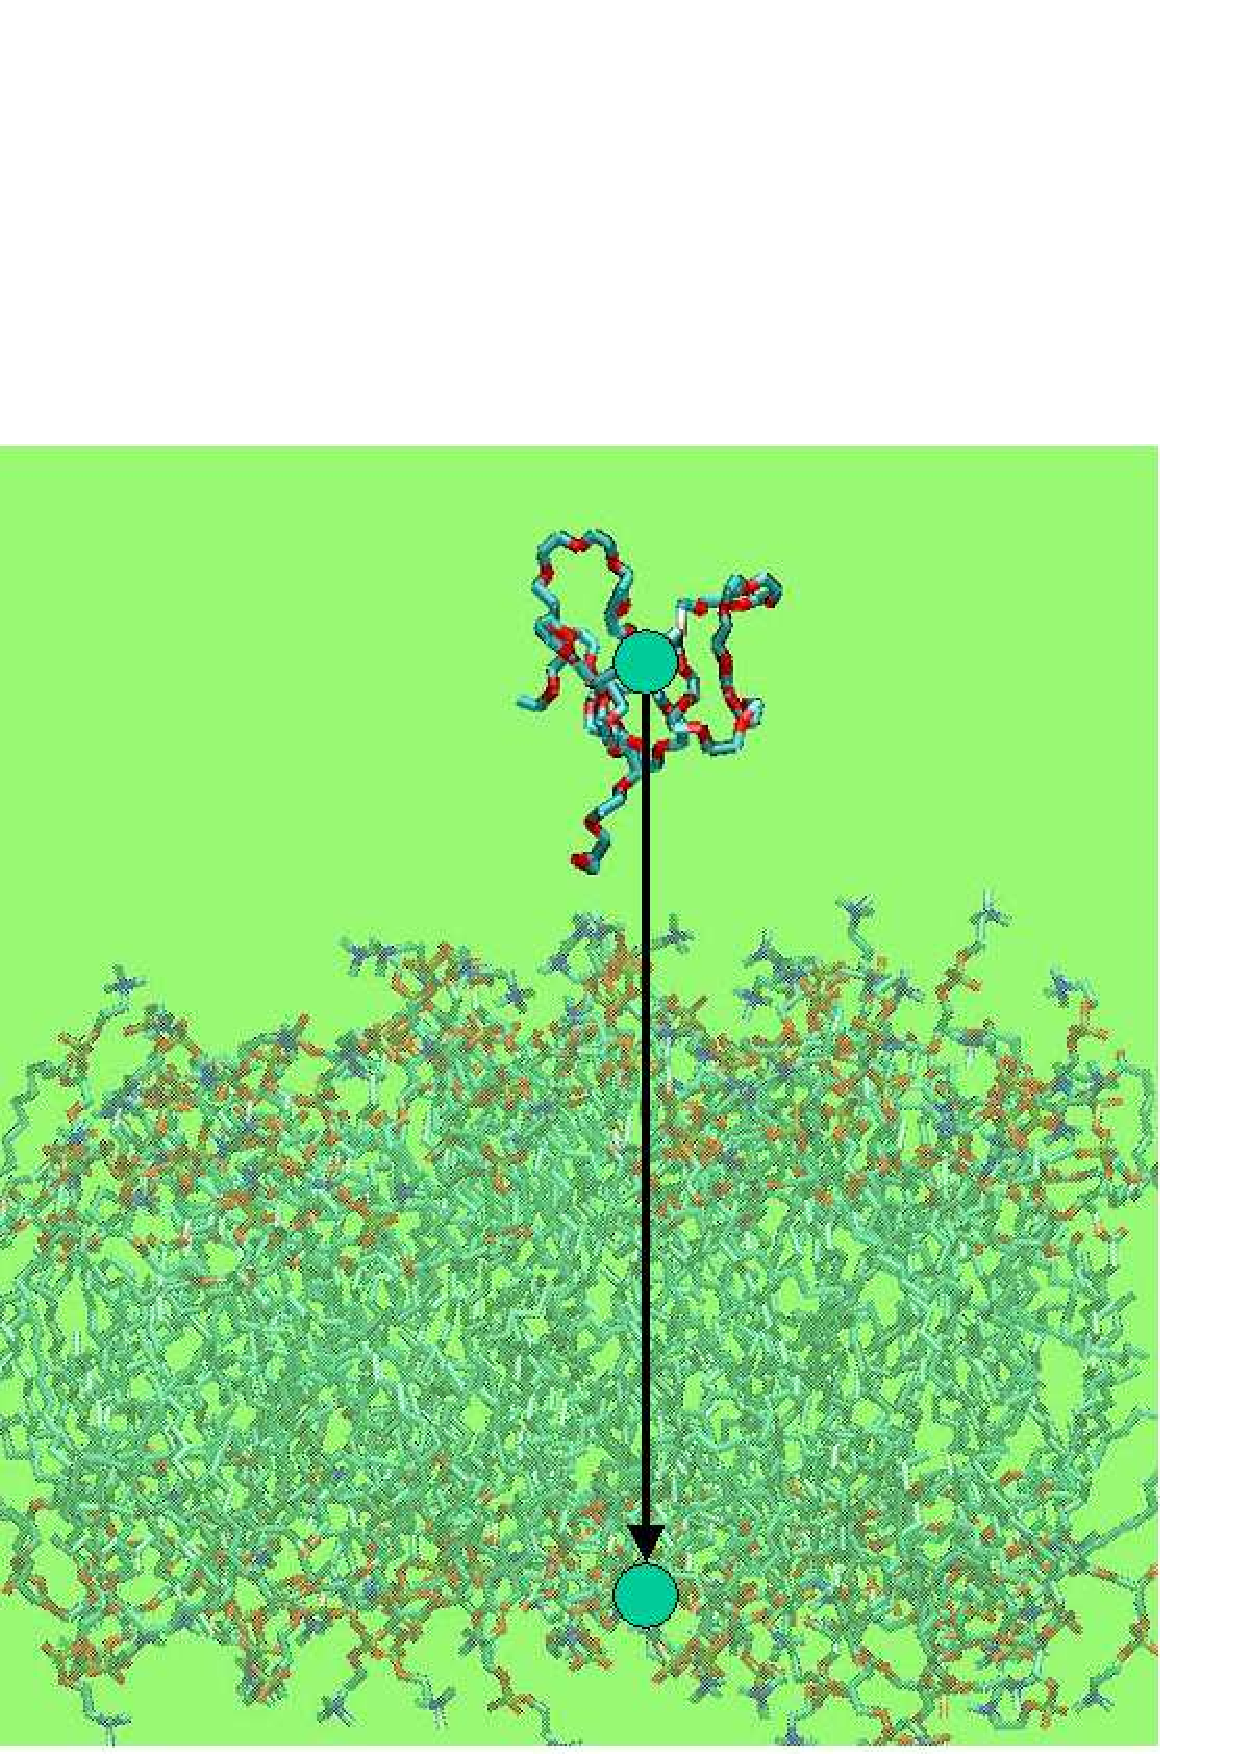
\includegraphics[width=6cm]{DrRoccatano-fig3}
    \caption{Schematic illustration of the steered molecular dynamics simulation experiment 
    for the pulling of the polymer into the membrane. The arrow represents the direction
    of the force applied on the polymer center of mass.}
    \label{fig:Roccatano3}
   \end{center}
\end{figure}


\item{} In collaboration with Dr. G. Milano and Dr. S. Pal (Biosystems Informatics 
Institute, Newcastle, UK), we published a simplified force 
field for polyethylenoxide (PEO)~\cite{Pal06}. The interactions of the polymer 
with a DMPC membrane and the barrier for the polymer penetration into the 
bilayer were evaluated using MD simulations and Steered Molecular Dynamics simulations 
(see Fig.\ref{fig:Roccatano3}). This new PEO model (and soon another 
new model for polypropilenoxide, PPO) will be applied to model triblocked polymers  
(PEO-PPO-PEO) micelle in contact with biological membranes. 

\item{} Finally, I was invited by Dr. A. V Zvelindovsky (University of Central Lancashire, Preston, UK)  
to write a book chapter on Molecular Dynamics Simulations for "Nanostructured Soft 
Matter: Experiment, Theory, Simulation and Perspectives". \cite{Roccatano06b}

\end{itemize}

\nocite{Schenk06,Wong06,Wong06b,Roccatano06a}
Danilo Roccatano is also involved in "Biotechnology".


\paragraph{Collaborations}
\begin{enumerate}
\item {\sl International University Bremen} \\ Prof. Ulrich Schwaneberg \\ Study of 
the organic solvent effects on
monooxygenase P450 BM-3 and Mutagenesis Assistant Program.
\item {\sl International University Bremen} \\ Prof. Werner M. Nau \\ Study of the 
dynamics in solution of small 
peptides by Molecular Dynamics simulation and time-resolved spectroscopic 
tecniques.
\item {\sl International University Bremen} \\ Prof. Martin Zacharias \\ Molecular 
Dynamics simulation study of the nucleosome core particle.
\item {\sl University of Salerno, Italy} \\ Dr. Giuseppe Milano \\ Interaction of 
polymer with biological membranes.
\item {\sl University of East Anglia, Norwich (UK)} \\ Dr. Steven Hayward \\ Theoretical 
investigation of domain motion in proteins.
\item {\sl Max Planck Institute for Biophysical Chemistry, Goettingen,Germany. } \\ 
Dr. Bert de Groot \\ Theoretical investigation of domain motion in proteins.
\end{enumerate}



